\documentclass[12pt]{kiarticle} % You can learn about my document class "kiarticle" and install it to your device by following the link: https://github.com/Kiarendil/toolkitex
\graphicspath{{pic/}}
\DeclareGraphicsExtensions{.pdf,.png,.jpg,.eps}
%%%
\pagestyle{fancy}
\fancyhf{}
%\renewcommand{\headrulewidth}{ 0.1mm }
\renewcommand{\footrulewidth}{ .0em }
\fancyfoot[C]{\texttt{\textemdash~\thepage~\textemdash}}
\fancyhead[L]{Лабораторная работа № 3.2.6 \hfil}
\fancyhead[R]{\hfil Иванов Кирилл, 625 группа }
\usepackage{multirow} % Слияние строк в таблице
\newcommand
{\un}[1]
{\ensuremath{\text{#1}}}
\newcommand{\eds}{\ensuremath{ \mathscr{E}}}


\begin{document}
	
	\begin{titlepage}
		\begin{center}
			\large 	Московский физико-технический университет \\
			Факультет общей и прикладной физики \\
			\vspace{0.2cm}
			
			\vspace{4.5cm}
			Лабораторная работа № 3.2.6 \\ \vspace{0.2cm}
			\large (Общая физика: электричество и магнетизм) \\ \vspace{0.2cm}
			\LARGE \textbf{Исследование гальванометра}
		\end{center}
		\vspace{2.3cm} \large
		
		\begin{center}
			Работу выполнил: \\
			Иванов Кирилл,
			625 группа
			\vspace{10mm}
			
			
			
			
		\end{center}
		
		\begin{center} \vspace{60mm}
			г. Долгопрудный \\
			2017 год
		\end{center}
	\end{titlepage}
	
	
	
	
	\paragraph*{Цель работы:} изучение работы высокочувствительного зеркального гальванометра магнитоэлектрической системы в режимах измерения постоянного тока и электрического заряда.
	
	\paragraph*{Оборудование:} зеркальный гальванометр с осветителем и
	шкалой, источник постоянного напряжения, делитель напряжения, магазин сопротивлений, эталонный конденсатор, вольтметр, переключатель, ключи, линейка.
	
	
	\section{Историческая справка}
	
	Гальванометром называют электроизмерительный прибор высокой
	чувствительности. С его помощью измеряют малые токи, напряжения,
	заряды, магнитные потоки. Выпускаются гальванометры различных си-
	стем: электромагнитные, магнитоэлектрические, электростатические и
	электродинамические. Наибольшее распространение получили гальвано-
	метры постоянного тока магнитоэлектрической системы. 
	
	В июне 1820 года Ганс Эрстед опубликовал описание опыта, для выполнения которого нужно:
	
	\begin{itemize}
		\item взять магнитную стрелку (стрелку, изготовленную из магнитного материала, часть магнитного компаса);
		\item	дождаться, пока направление стрелки совпадёт с направлением магнитного меридиана Земли;
		\item	установить над стрелкой прямолинейный проводник так, чтобы проводник располагался вдоль магнитного меридиана Земли;
		\item	начать пропускать через проводник электрический ток.
	\end{itemize}

	Результат: стрелка отклонится от направления магнитного меридиана Земли.
	
	
	Для усиления действия тока Иоганн Швайггер:
	
	\begin{itemize}
		\item намотал на прямоугольную рамку несколько витков проводника;
		\item поместил магнитную стрелку внутрь прямоугольной рамки.
	\end{itemize}

	Полученное устройство получило название «мультипликатор» и было продемонстрировано в университете Галле 16 сентября 1820 года. «Мультипликатор» Швейггера можно считать первым гальванометром (точнее, гальваноскопом).
	
	Термин «гальванометр» впервые появился в 1836 году, произошёл от фамилии учёного Луиджи Гальвани.
	
	
	\section{Теоретическое введение}
	
	\begin{wrapfigure}{l}{0.35\linewidth} 
		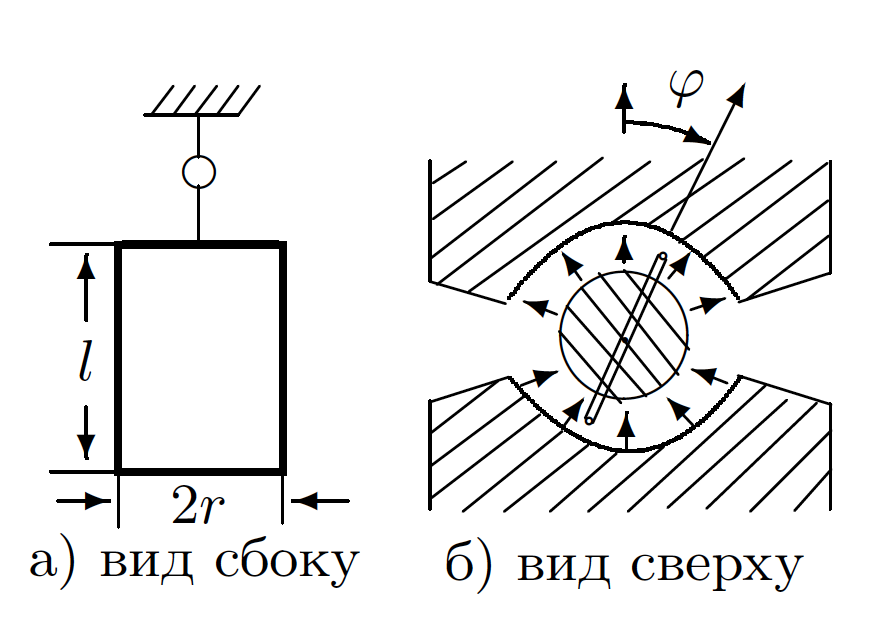
\includegraphics[width=6cm]{ramka}
		\caption{Рамка}
		\label{}
	\end{wrapfigure}

Главной частью высокочувствительного гальванометра магнитоэлектрической системы является подвешенная на вертикальной нити рамка, помещённая в поле постоянного магнита (рис. 1). Вырез цилиндрической формы в полюсах магнита и ферромагнитный цилиндр на оси системы делают поле в зазоре радиальным. Скреплённое с рамкой зеркальце служит для измерения угла поворота рамки. Магнит и подвижная система заключены в защитный кожух.

Запишем основное уравнение колебаний рамки:

\begin{equation}\label{main}
\ddot{\phi} + 2\gamma\dot{\phi }+ \omega_0^2\phi = K I
\end{equation}
	
	где введены обозначения: $ 2\gamma = \dfrac{(BSN)^2}{JR_\Sigma} $, $ \omega_0^2 = \dfrac{D}{J}, K = \dfrac{BSN}{J} $. Эти величины выражены через параметры установки: $ B $ --- магнитное поле, в которое помещена рамка, $ I  = \dfrac{\eds}{R_\Sigma}$ --- ток, текущий через рамку, $ R_\Sigma $ --- сопротивление рамки и цепи, $ N $ --- число витков рамки, $ S $ --- площадь витка рамки, $ J $ --- момент инерции системы, $ D $ --- модуль кручения нити.
	
	\subsection{Стационарный режим}
	Если через рамку пропускать постоянный ток (достаточно дол-
	го, чтобы затухли колебания подвижной системы), то в уравнении \eqref{main} можно положить $ \ddot{\phi} = \dot{\phi } = 0 $, и угол поворота определится формулой
	
	\begin{equation}\label{C1}
	\phi = \dfrac{I}{C_1}, \qquad C_I = \dfrac{D}{BSN} = \dfrac{I}{\phi}
	\end{equation}
	
	где $ C_I $ --- динамическая постоянная гальванометра.
	
	\subsection{Свободные колебания}
	
	При отсутствии внешнего источника тока, мы получаем, что левая часть уравнения \eqref{main} равна нулю. Это обычное уравнение колебаний, решение и свойства которого рассматривались в курсе механики и прошлой работе 3.2.4., не будем останавливаться на нем подробно, напомним лишь, что в зависимости параметра $ \gamma $ у нас есть колебательный режим, критический режим и случай переуспокоенного гальванометра, причем в последних двух случаях движение апериодическое. 
	
	\subsection{Баллистический режим}
	
	Период свободных колебаний баллистического гальванометра благодаря искусственному увеличению момента инерции рамки оказывается очень большим (порядка десяти секунд). Если пропустить через рамку короткий импульс тока, то можно считать, что весь ток успевает пройти при неотклоненном положении рамки. Рамка, однако, при этом получает толчок, в результате которого возникает движение, описываемое уравнением свободных колебаний при начальных условиях $ \phi(t) = 0, \dot{\phi }(0) = \dot{\phi }_0 $.

	Для вычисления скорости $ \dot{\phi }_0 $, полученной в результате толчка, умножим уравнение \eqref{main} на $ dt $ и проинтегрируем его по времени от 0 до момента окончания токового импульса $ \tau $. Пренебрегая малыми вторым и третьим членом в левой части, получаем,
	
	\begin{equation}\label{q}
	\int\limits_0^\tau \ddot{\phi}dt = K 	\int\limits_0^\tau I dt \te \dot{\phi }(\tau) = Kq
	\end{equation}
	
	где $ q $ --- полный электрический заряд, прошедший через рамку за время импульса. При этом мы пренебрегаем зарядом индукционного тока.
	
	
	Величина $ C_Q = \dfrac{q}{\phi_{max}}$ называется баллистической постоянной гальванометра. Баллистическая постоянная наряду с динамической является важнейшей характеристикой гальванометра, но в отличие от динамической она существенно зависит от режима работы гальванометра (от сопротивления цепи).
	
	Расчёт показывает, что максимальный отброс достигается при полном
	отсутствии затухания (тормозящий индукционный ток отсутствует при
	обрыве в цепи):
	
	\begin{equation}\label{}
	\phi_{max \; св} = \dfrac{\dot{\phi }(\tau) }{\omega_0} = \dfrac{Kq}{\omega_0}
	\end{equation}
	
	В этом случае, однако, возникшие в результате отброса колебания рам-
	ки не будут успокаиваться, и прибор не скоро сможет быть использован
	для повторных измерений.
	
	Обычно удобнее всего работать в режиме, близком к критическому:
	
	\begin{equation}\label{}
	\phi_{max \; кр} = \dfrac{Kq}{\omega_0 e}
	\end{equation}
	
	Таким образом, в критическом режиме максимальное отклонение зайчика в $ e $ раз меньше, чем в режиме свободных колебаний. Отсюда, в частности,  следует, что отношение баллистических постоянных
	
	\begin{equation}\label{}
	\dfrac{C_{Q \; кр}}{C_{Q \; св}} = e
	\end{equation}
	
	
	
	\section{Экспериментальная установка}

	\subsection{Стационарный ток}
	
	В режиме стационарного тока можно легко вычислить ток по формуле 
	
	\begin{equation}\label{I}
	I = U_0 \dfrac{R_1}{R_2} \dfrac{1}{R + R_0}
	\end{equation}
	
	Координата $ x $ зайчика связана с углом $ \phi $ простым соотношением $ x = a\tg 2\phi $, и при малых $ \phi  =  \dfrac{x}{2a}$, где $ a $ --- расстояние от шкалы до зеркальца. 
	
	Отсюда из \eqref{C1} получаем:
	
	\begin{equation}\label{C1exp}
	C_I = \dfrac{2aI}{x}
	\end{equation}
	
			\begin{wrapfigure}{l}{0.65\linewidth} 
		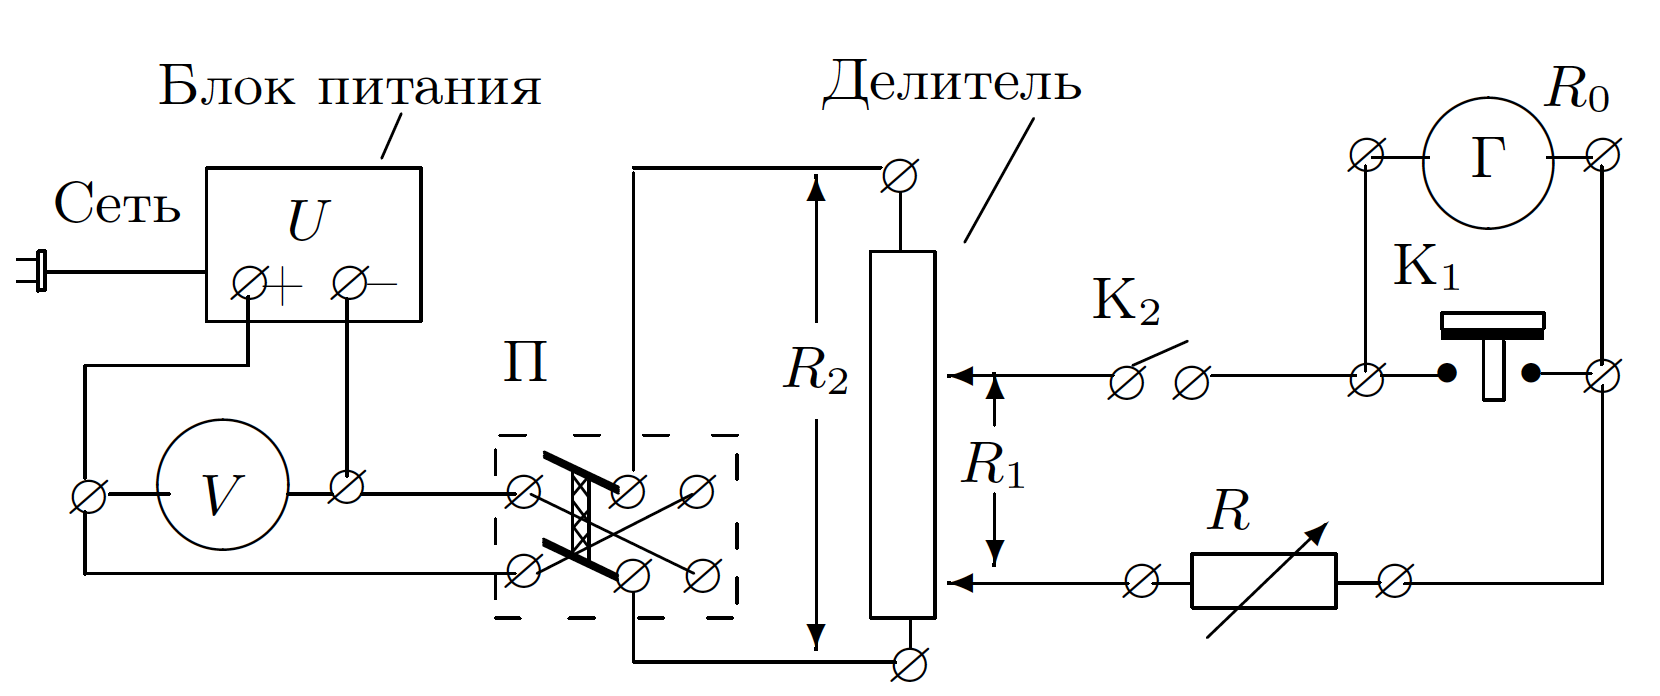
\includegraphics[width=10cm]{scheme1}
		\caption{Схема установки для первой и второй частей работы}
		\label{chain1}
	\end{wrapfigure}
	
	\subsection{Критический режим и свободные колебания}
	
	Логарифмический декремент затухания определяется экспериментально по формуле
	
	\begin{equation}\label{Theta}
	\Theta =  \gamma T =  \ln \dfrac{x_k}{x_{k+n}}
	\end{equation}
	
	При этом мы можем выразить декремент как
	
	\begin{equation}\label{}
		\Theta =  \gamma T =  \dfrac{2\pi\gamma}{\sqrt{\omega_0^2 - \gamma^2}} = \dfrac{2\pi R_3}{\sqrt{(R + R_0)^2 - R_3^2}}
	\end{equation}
	
	где $ R_3 = R_{кр} + R_0 $. Отсюда нетрудно получить формулу: 
	
	\begin{equation}\label{}
	\dfrac{4\pi^2}{\Theta^2} = \dfrac{(R_0 + R)^2}{(R_0 + R_{кр})^2} - 1
	\end{equation}
	
	Для расчета $ R_{кр} $ будем использовать следующую формулу:
	
	\begin{equation}\label{Rkr}
	R_{кр} = \dfrac{R + R_0}{1 + \frac{4\pi^2}{\Theta^2}} - R_0 = \co
	\end{equation}
	 
	 Таким образом, отношение $ f(R) $ и $ F(\Theta) $ из физического смысла должно быть постоянным. 
	 
	 \subsection{Баллистический режим}
	 \begin{wrapfigure}{l}{0.65\linewidth} 
	 	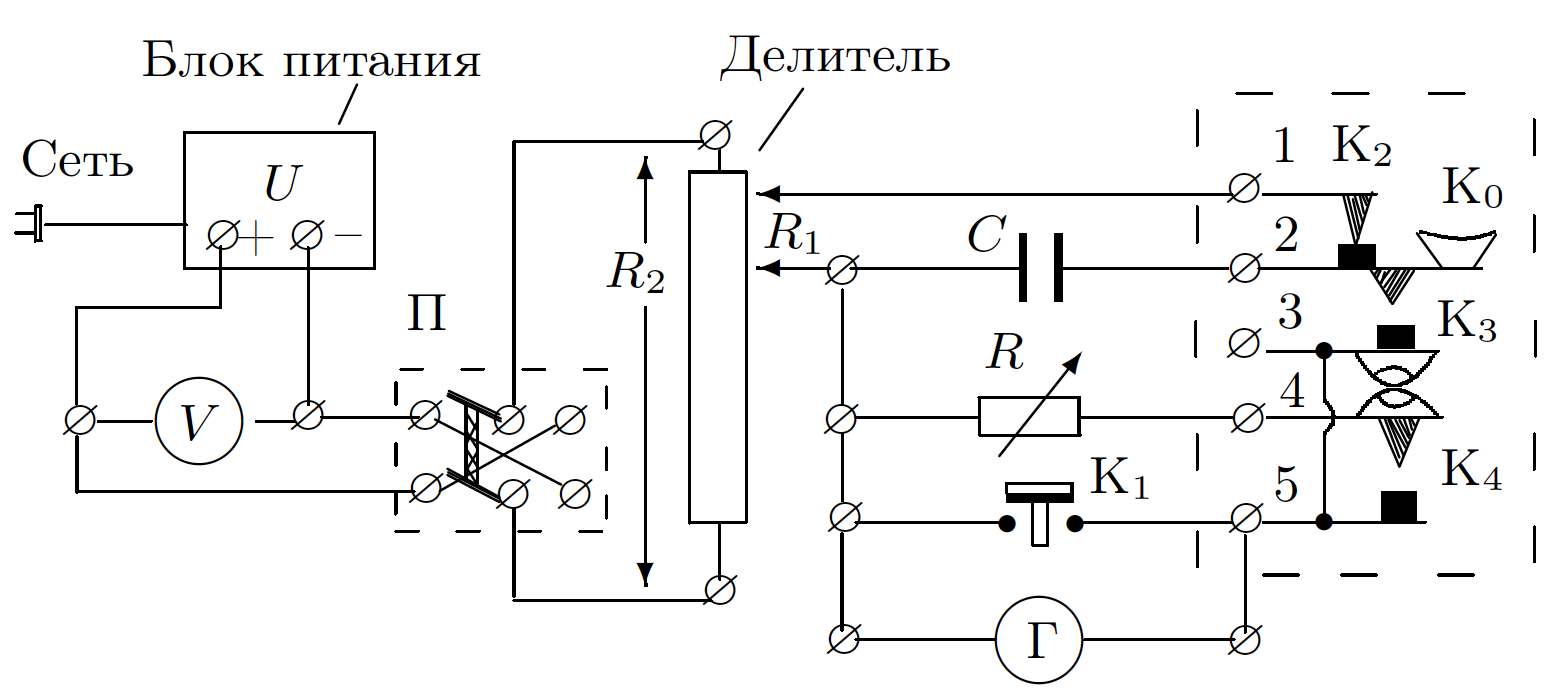
\includegraphics[width=10cm]{scheme2}
	 	\caption{Схема установки для третей части работы}
	 	\label{chain2}
	 \end{wrapfigure}
	 
	 Заряд конденсатора $ C $ равен 
	 
	 \begin{equation}\label{}
	 q = U_C C = C \dfrac{R_1}{R_2}U_0
	 \end{equation}
	 
	 Из решения уравнения колебаний и формулы декремента следует формула 
	 
	 \begin{equation}\label{}
	 l_0 = l_1 e^{\Theta/4}
	 \end{equation}
	 
	 При сопротивлении, равном критическому, баллистическая постоянная будет определяться
	 
	 \begin{equation}
	 C_{Q кр} = \dfrac{q}{\phi_{max \; кр}} = 2a\dfrac{R_1}{R_2}\dfrac{U_0C}{l_{max \; кр}}
	 \label{C}
	 \end{equation}
	 
	 \section{Ход работы}
	 
	 \subsection{Динамическая постоянная}
	 
	 	 \begin{table}[h]
	 	\centering
	 	\caption{Результаты измерений при стационарном режиме}
	 	\begin{tabular}{|c|c|c|c|c|c|}
	 		\hline
	 		№ & $ R $, кОм & $ x $, см & $ \sigma_x $ & $ I, 10^{-8} $ А & $ \sigma_I, 10^{-8} $ А\\
	 		\hline
	 		1 & 20 & 21.6 & 0.2 & 9.92 & 0.10 \\
	 		2 & 23 & 19.0 & 0.2 & 8.66 & 0.09 \\
	 		3 & 26 & 16.7 & 0.2 & 7.68 & 0.08 \\
	 		4 & 29 & 15.1 & 0.2 & 6.90 & 0.07 \\
	 		5 & 32 & 13.8 & 0.2 & 6.27 & 0.06 \\
	 		6 & 35 & 12.6 & 0.2 & 5.74 & 0.06 \\
	 		7 & 38 & 11.6 & 0.2 & 5.29 & 0.05 \\
	 		8 & 41 & 10.8 & 0.2 & 4.91 & 0.05 \\
	 		9 & 45 & 9.9 & 0.2 & 4.48 & 0.04 \\
	 		10 & 50 & 9,0 & 0.2 & 4.03 & 0.04 \\
	 		11 & 60 & 7.6 & 0.2 & 3.37 & 0.03 \\
	 		12 & 70 & 6.5 & 0.2 & 2.89 & 0.03 \\
	 		\hline
	 	\end{tabular}% 
	 	\label{resI}% 
	 \end{table}% 
	 
	 \begin{figure}[h]
	 	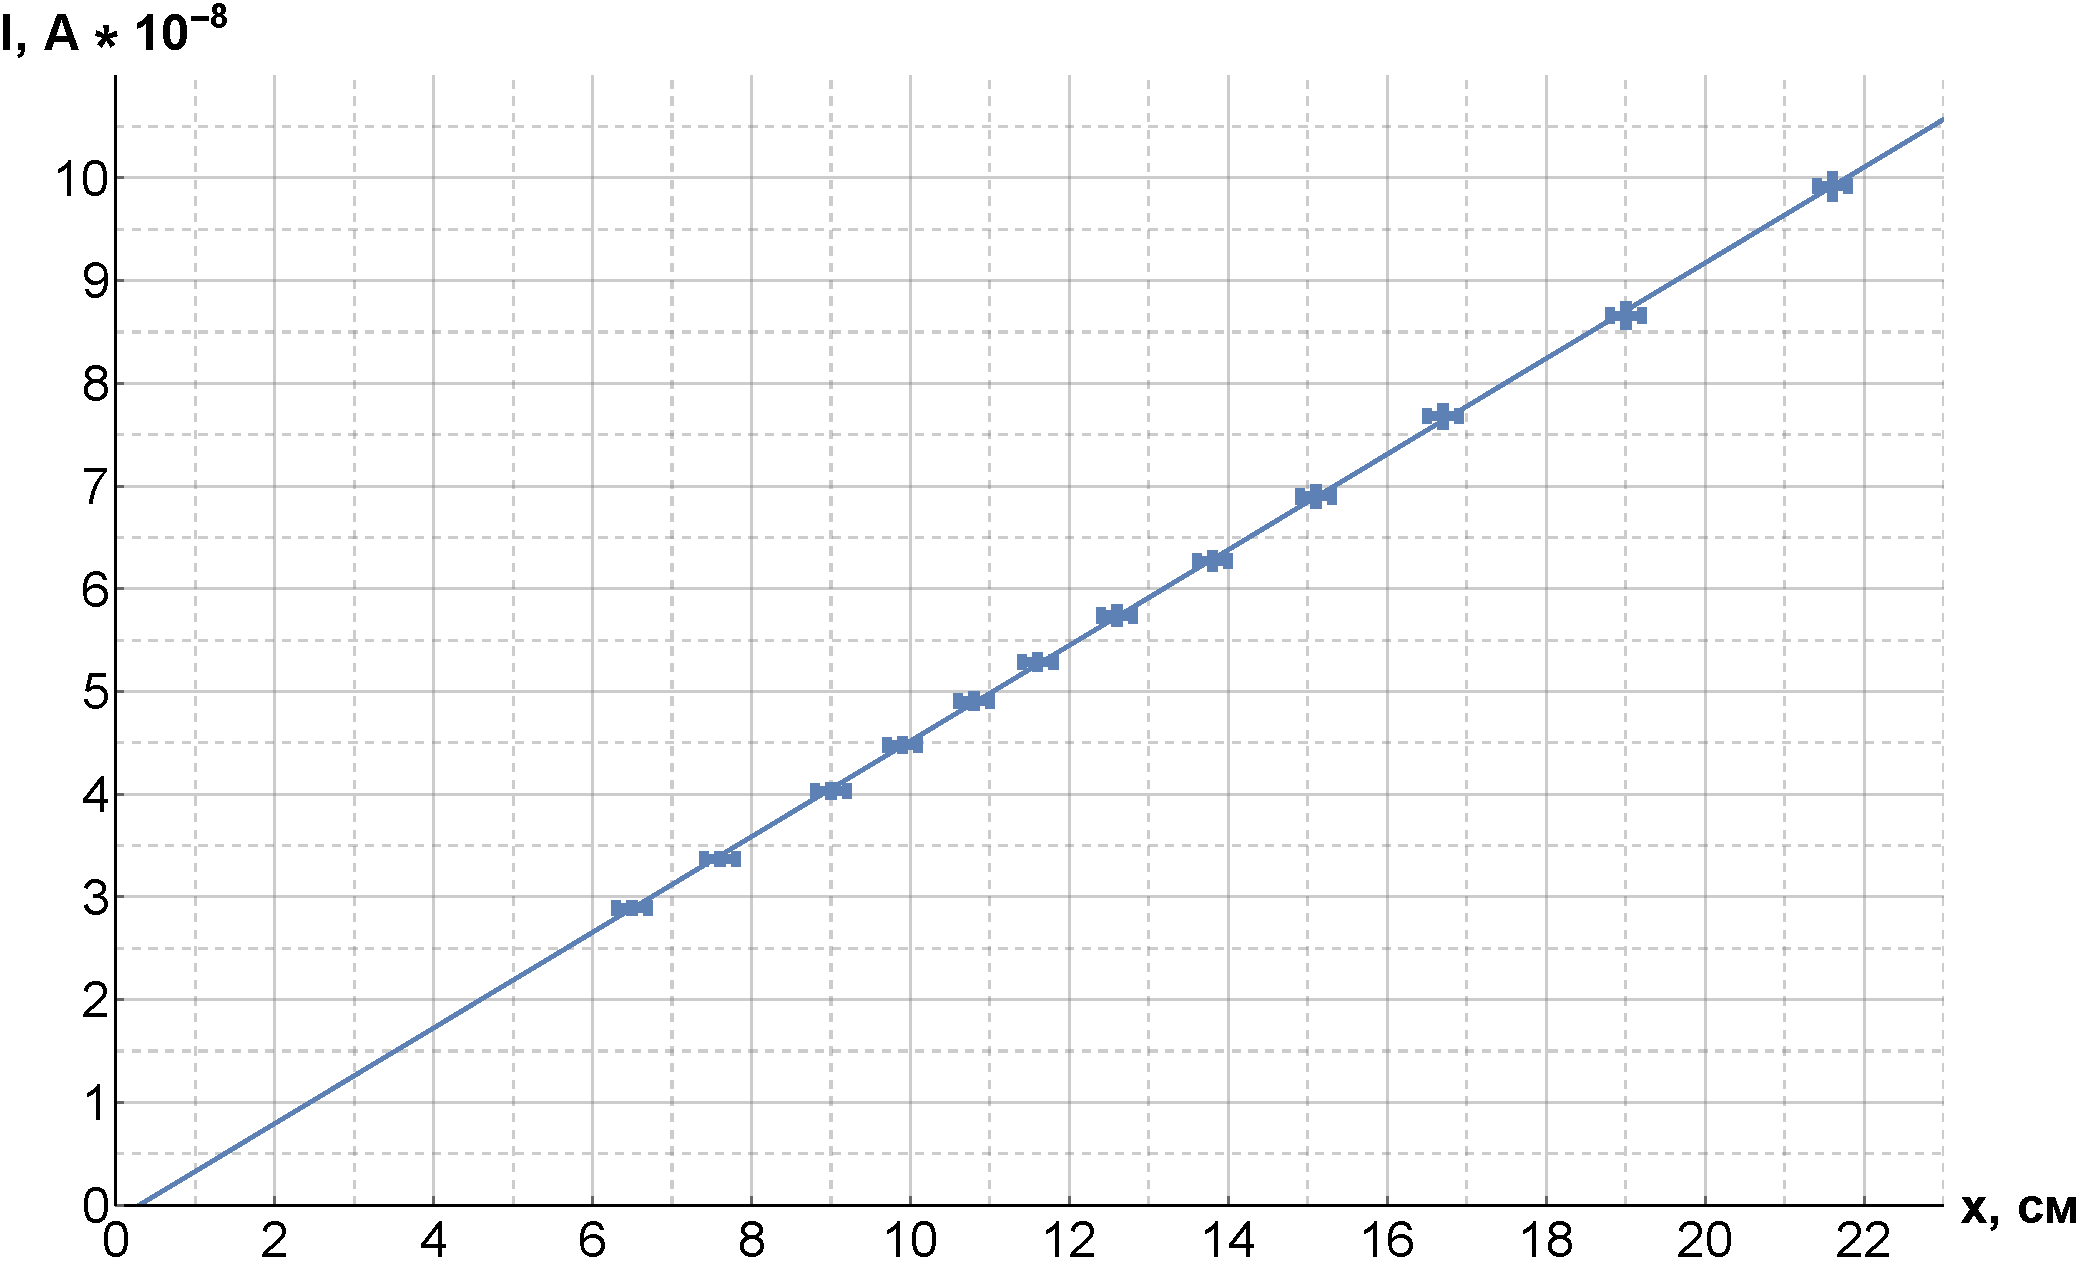
\includegraphics[scale=0.47]{Ix.pdf}
	 	\caption{Зависимость $ I $ от $ x $}
	 \end{figure}
	 
	 \begin{table}[h]%{l}{0.5\linewidth}
	 	\centering
	 	\caption{Расчет апроксимированной прямой $ y = ax +b $}
	 	\begin{tabular}{c|cc}
	 		\text{} & \text{Estimate} & \text{Standard Error} \\
	 		\hline
	 		a & 0.461 & 0.007 \\
	 		b & -0.060 & 0.010  \\
	 	\end{tabular}
	 	\label{y(x)}
	 \end{table}
	 
	 Соберем цепь рис. \ref{chain1}. Постоянные установки: $ U_0 = 2,04 \pm 0,02 $ В, $ R_2 = 10 $ кОм, $ R_0 = 560 $ Ом, $ a = 1,04 \pm 0,5 $ см. Установим делитель на положение $ 1/1000 $ и снимем зависимость отклонения зайчика от положения равновесия при изменении магазина сопротивлений. Подчитаем также ток по формуле \eqref{I}. Результаты занесем в таблицу \ref{resI}. 
	 
	 Построим график зависимости тока $ I $ от отклонения зайчика $ x $. Аппроксимируем полученный результат, занеся полученные данные в таблицу \ref{y(x)}. Получаем, что тангенс наклона равен $ \tg\alpha(0,461 \pm 0,007) \x 10^{-8} \frac{A}{см} $. Тогда по формуле \ref{C1exp} подсчитаем значение нашей постоянной: $ C_I = 2a\tg\alpha =  95,9 \x 10^{-8} $ А = $ 95,9 \x 10^{-5}  \dfrac{A}{\un{мм/м}}$. Ее погрешность высчитаем по формуле
	 
	 \begin{equation}\label{}
	 \dfrac{\sigma_{C_I}}{C_I} = \sqrt{ \left( \dfrac{\sigma_a}{a}\right)^2 + \left( \dfrac{\sigma_{\tg\alpha}}{\tg\alpha}\right)^2} \approx 0,006 
	 \end{equation}
	 
	 Тогда запишем итоговый ответ: 
	 
	 \begin{center}
	 	{\fbox{ $ С_I = (96,9 \pm 0,6 ) \x 10^{-8}  A =  (95,9 \pm 0,6 ) \x 10^{-5}  \dfrac{A}{\un{мм/м}} $ }} \\
	 \end{center} 
	 
	 	 


\subsection{Критическое сопротивление}

Измерим 2 последовательных отклонения зайчика при разомкнутом контуре:

\begin{itemize}
	\item $ x_n = 18,3 \; см, \quad x_{n+1} = 14,0 \; см $
		\item $ x_n = 19,2 \; см, \quad x_{n+1} = 14,9 \; см $
			\item $ x_n = 19,0 \; см, \quad x_{n+1} = 14,7 \; см $
\end{itemize}

Тогда мы получаем, что логарифмический декремент $ \Theta_0  = \dfrac{1}{3} \sum_1^3 \left( \ln \dfrac{x_n}{x_{n+1}}\right)_i  = 0,26 \pm 0,01 $ (погрешность получена среднеквадратичным отклонением). 

Измерим время $ n $ колебаний:
\begin{itemize}
	\item $ n = 3 \; см, \quad t = 15,3 \; с $
	\item $ n = 4 \; см, \quad t = 20,1 \; с $
	\item $ n = 3 \; см, \quad t = 15,1 \; с $
\end{itemize}

Тогда мы получаем, что период колебаний примерно равен $ T_0  = \dfrac{1}{3} \sum_1^3 \left( \dfrac{t}{n} \right)_i \approx 5,05 \hm{\pm} 0,03\; с$ (погрешность получена среднеквадратичным отклонением).

Определим критическое сопротивление. Для этого подберем наибольшее сопротивление магазина, при котором при размыкании ключа $ П $ зайчик не переходит за нулевое значение. Примерно получаем $ R_{кр} = 8 \pm 0,1 кОм $. 

Теперь для расчёта $ \Theta $  проведём измерение отклонений зайчика после размыкания ключа $ П $, увеличивая $ R $ магазина от примерно $ 3R_{кр} $  до 1$ 0R_{кр} $. Подсчитаем при этом логарифмический декремент по формуле \eqref{Theta} и отношение для расчёта $ R_{кр} $ по формуле \eqref{Rkr}. Результаты сведем в таблицу \ref{resR}:

\begin{table}[h]
	\centering
	\caption{Результаты измерений при свободных колебаниях}
	\begin{tabular}{|c|c|c|c|c|c|}
		\hline
		$ N $& $ R, \; кОм $& $ x_n, $ см &$ x_{n+1}, $ см & $ \Theta $ & $ R_{кр} $, кОм\\
		\hline
		1 & 24 & 5.9 & 0.8 & 2.00 & 6.89 \\
		2 & 28 & 11.1 & 1.7 & 1.88 & 7.62 \\
		3 & 32 & 10.6 & 1.6 & 1.67 & 7.81 \\
		4 & 36 & 10.3 & 2.4 & 1.46 & 7.70 \\
		5 & 40 & 10.2 & 2.7 & 1.33 & 7.84 \\
		6 & 44 & 9.8 & 3.0 & 1.18 & 7.69 \\
		7 & 48 & 9.8 & 3.2 & 1.12 & 7.96 \\
		8 & 56 & 14.4 & 5.3 & 1.00 & 8.33 \\
		9 & 64 & 13.0 & 5.2 & 0.92 & 8.76 \\
		10 & 72 & 12.0 & 5.2 & 0.84 & 9.02 \\
		11 & 80 & 11.8 & 5.5 & 0.76 & 9.16 \\
		\hline
	\end{tabular}% 
	\label{resR}% 
\end{table}% 

Видно, что $ 2-7 $ точки примерно равны, тогда подсчитаем для них истинное среднее с помощью распределения Стьюдента: 

\begin{equation}\label{}
R_{кр} = \langle R_{кр \; т}\rangle \pm A \dfrac{\sigma_R}{\sqrt{N}}
\end{equation} 

Где $ A = 2,015 $ --- коэффициент Стьюдента, $   \langle R_{кр \; т}\rangle = 7,78 $ кОм --- среднее арифметическое точек $ 2-7 $, $ \sigma_R  = 0,13 $ кОм --- среднеквадратичное отклонение. $ N = 6 $. Получаем ответ: 

	 \begin{center}
	{\fbox{ $ R_{кр} = 7,78 \pm 0,10 \; кОм $ }} \\
\end{center} 

\subsection{Баллистическая постоянная}

 \begin{table}[h]
	\centering
	\caption{Результаты измерений при динамическом режиме}
	\begin{tabular}{|c|c|c|c|}
		\hline
	$ N $ & $ R, $ кОм & $ \dfrac{1}{R+R_0}, 10^{-6}\; Ом^{-1} $& $ l_{max}, см $ \\
		\hline
		1 & 50 & 19.8 & 21.4 \\
		2 & 45 & 21.9 & 20.3 \\
		3 & 40 & 24.7 & 19.6 \\
		4 & 30 & 32.7 & 18.4 \\
		5 & 20 & 48.6 & 16.6 \\
		6 & 15 & 64.3 & 15.2 \\
		7 & 10 & 94.7 & 13.2 \\
		8 & 8 & 116.8 & 12.0 \\
		9 & 6 & 152.4 & 10.4 \\
		10 & 4 & 219.3 & 8.6 \\
		11 & 3 & 280.9 & 7.4 \\
		12 & 2.5 & 326.8 & 7.0  \\
		\hline
	\end{tabular}% 
	\label{resL}% 
\end{table}% 

	 \begin{figure}[h!]
	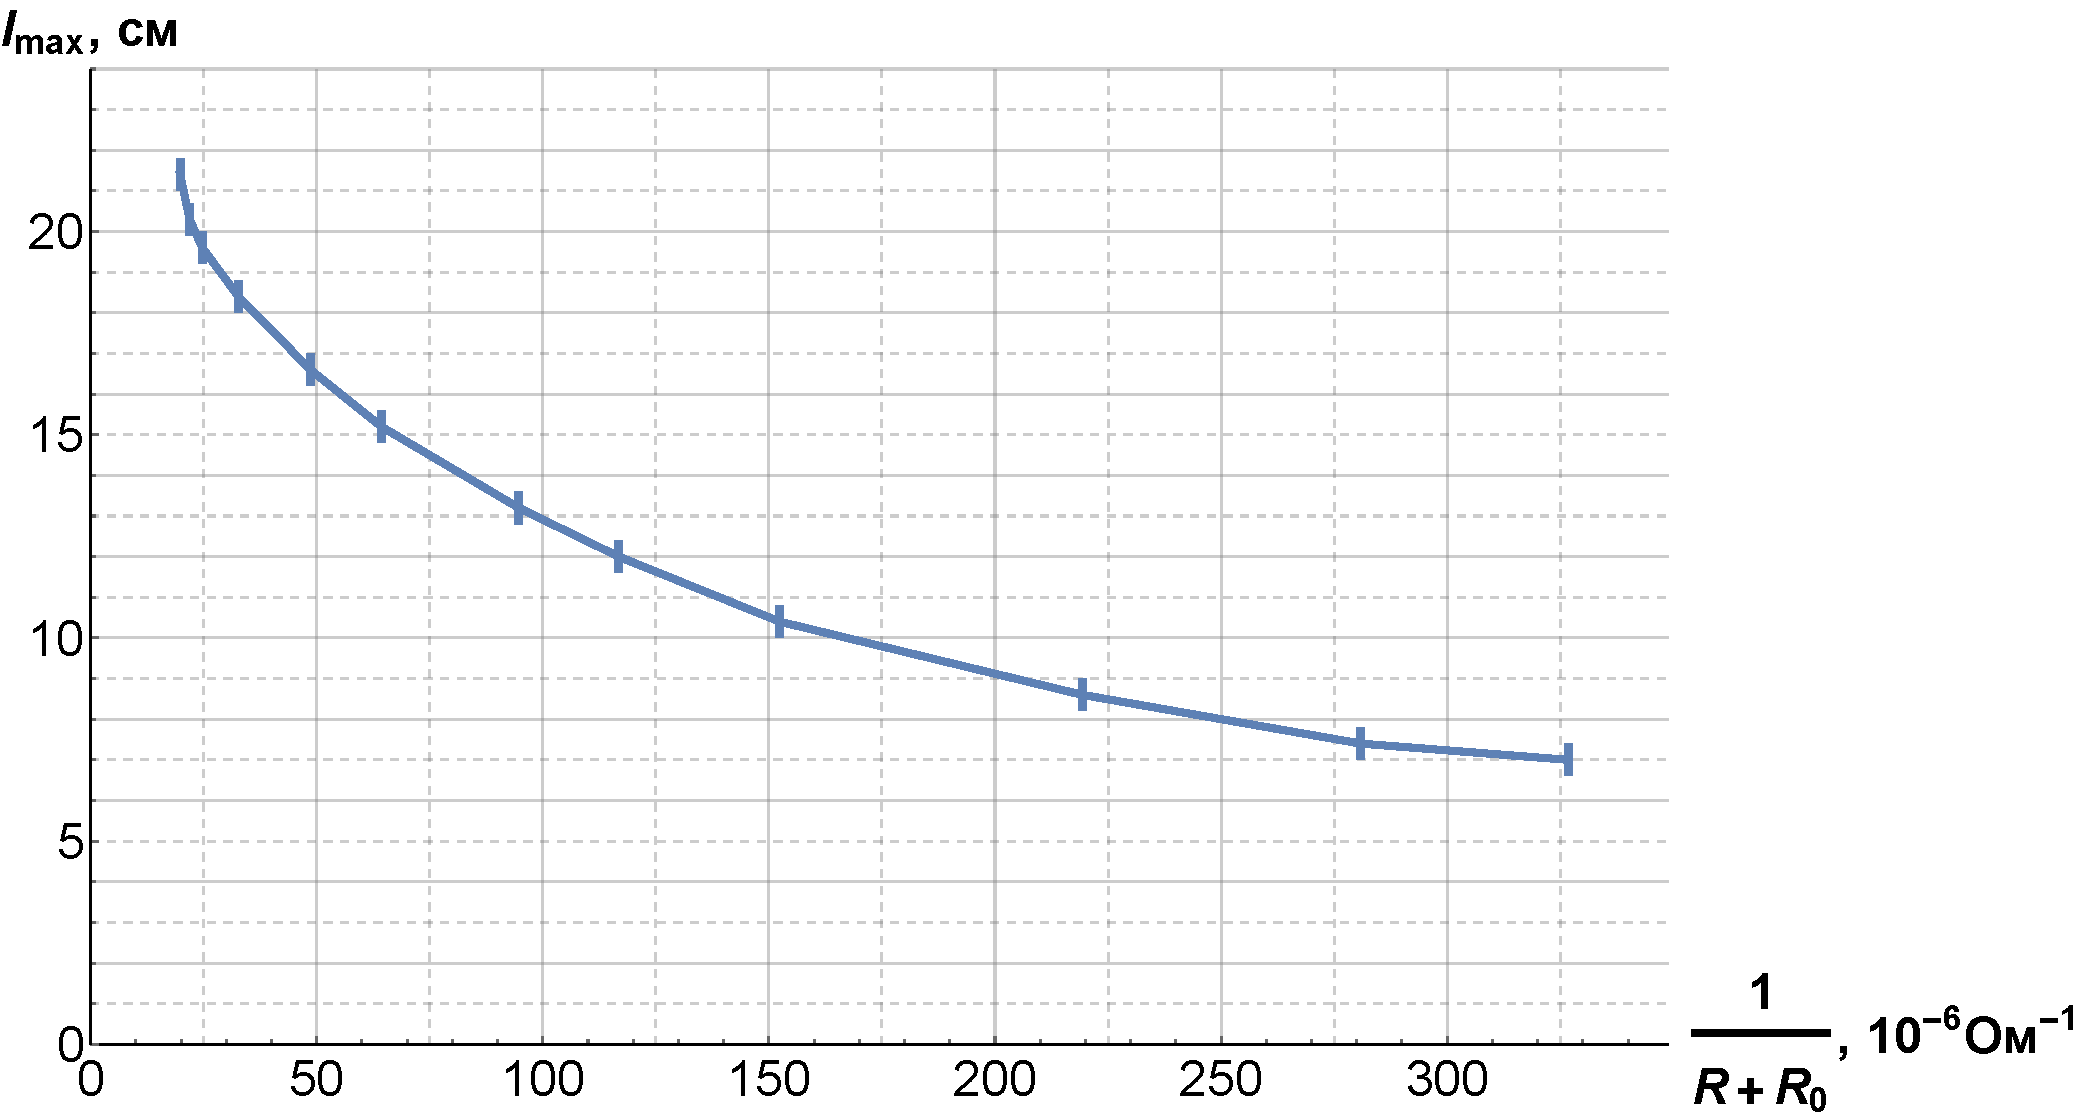
\includegraphics[scale=0.5]{L.pdf}
	\caption{График зависимости $ l_{max} $ от $ \dfrac{1}{R + R_0} $}
\end{figure}

Теперь соберем схему согласно рис.\ref{chain2}. Емкость конденсатора $ C = 2  $ мкФ. Установив делитель на положение 1/40, найдем такое первое отклонение зайчика после замыкания $ K_0 $, при котором он занимает всю шкалу, а именно $ l_{0} =  24,4 \pm 0,3 $ см. Теперь не меняя положения делителя, снимем зависимость первого отклонения от величины $ R $.  Найдем величину $ \dfrac{1}{R + R_0} $ и результаты сведем в таблицу \ref{resL}. Теперь построим график зависимости $ l_{max} $ от величины $ \dfrac{1}{R + R_0} $.  

Найдем величину $ l_1 = l_0 e^{\Theta_0/4} = 26, 0 $ см. Величина, в $ e $ раз меньшая, это $ l_e = 9,6 $ см. На графике видно, что этой точке соответствует величина $ 180 \x10^{-6} \;Ом^{-1} = \dfrac{1}{R+R_0}$. Получаем:

\begin{equation}\label{}
R + R_0 = \dfrac{1}{180 \x10^{-6}} \te R = \dfrac{10^6}{180} - 560\approx 5,0 \; кОм.
\end{equation}

Теперь найдем баллистическую постоянную  по формуле \eqref{C}:

\begin{equation}\label{}
С_{Q_{кр}} = 2a \dfrac{R_1}{R_2} \dfrac{U_0C}{l_e} = 2,22 \x 10^{-6} \; Кл
\end{equation}

Подсчитав погрешность по формуле 

\begin{equation}\label{}
\sigma_{С_{Q_{кр}} } = С_{Q_{кр}} \sqrt{ \left( \dfrac{\sigma_U}{U_0} \right)^2+ \left( \dfrac{\sigma_a}{a} \right)^2 + \left( \dfrac{\sigma_{l_e}}{l_e}\right)  } = 0,03 \x 10^{-6} \; Кл
\end{equation}

Тогда получаем ответ:

	 \begin{center}
	{\fbox{ $С_{Q_{кр}}  =  (2,22 \pm 0,03) \x 10^{-6} \; Кл  = (2,22 \pm 0,03) \x 10^{-3} \; \dfrac{Кл}{мм/м}  $ }} \\
\end{center} 

Подсчитаем время релаксации и сравним с периодом свободных колебаний:

\begin{equation}\label{}
\tau = R_0C \approx 1, 1 \; мс \quad \te \quad \dfrac{T}{\tau} \approx 4,5 \x 10^3
\end{equation}

\subsection{Вывод}

Итак, в этой работе мы изучили работу гальванометра в трех режимах: стационарном, свободных колебаний и баллистическом. Мы измерили критическое сопротивление контура $ R_{кр} $ тремя способами, а также нашли динамическую и баллистическую постоянную установки. 

Результаты сведем в табличку:

\begin{table}[h!]%{l}{0.5\linewidth}
	\centering
	\caption{Итоговые результаты: }
	\begin{tabular}{|c|c|c|c|c|c|c|}
		\hline
			\multirow{2}{*}{$ N $} & 		\multirow{2}{*}{$ R_0,\; Ом $} & \multicolumn{3}{|c|}{$ R_{кр} $} & 	$ C_I, $ & 	$С_{Q_{кр}},$ \\
		\cline{3-5}
		& &Подбор & $ \dfrac{1}{\Theta^2} $ & Балл. & $ 10^{-5} \dfrac{A}{\un{мм/м}}   $ & $ 10^{-3}  \dfrac{Кл}{мм/м}  $ \\
%		\multirow{2}{*}{$  L $} & \multicolumn{3}{|c|}{$ R_{кр} $} \\
%		\cline{2-4}
%		& Теор. & Подбор & Граф.  \\
%		\hline
%		$ 393 \pm  7 $ мГн   & $ 17,73 \pm 0,33 $ кОм & 12,6 кОм & 	$ 17,71 \pm 0,31 $ кОм \\
		\hline
		&  560 &  $ 8,0 \pm 0,1  $ кОм &  $ 7,78 \pm 0,10 \; кОм $& $ 5, 0 $ кОм& $ 96,9 \pm 0,6  $& $ 2,22 \pm 0,03 $ \\
		\hline
	\end{tabular}
\end{table}
 	 
 	\end{document}